\documentclass[10pt]{article}
\usepackage{fullpage}
\usepackage{amsmath,amssymb, tikz}
\usepackage{amsthm,xcolor, dsfont}
\usepackage{tikz}
\usetikzlibrary{arrows}
\setlength{\parindent}{0pt}

\begin{document}
\begin{center}
\textbf{\Large{HW 4 - Group Actions on $B_n$ (Due Thursday 2/29)}}
\end{center}
\medskip

\textbf{0}. [\textbf{Warm-up}; \textbf{Not-for-credit}] Draw the Hasse diagram of the poset of nonisomorphic simple graphs with $5$ vertices (with subgraph containment ordering). What is the size of the largest antichain ? How many antichains have this size ?\\

\textbf{1}. [\textcolor{red}{Some (counter)-examples}]\smallskip

$(i)$ Give an example of a finite graded poset $P$ with the Sperner property, together with a group $G$ acting on $P$, such that $P/G$ is \emph{not} Sperner (From our lectures we know that $P$ cannot be $B_n$)\medskip

$(ii)$ Consider the poset $P$ whose Hasse diagram is given by

\begin{center}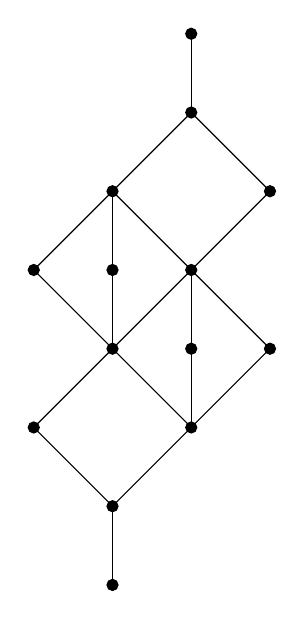
\begin{tikzpicture}
\draw[fill=black] (0,-0.5) circle (2pt);
\draw[fill=black] (0,0.5) circle (2pt);
\draw[fill=black] (-1,1.5) circle (2pt);
\draw[fill=black] (1,1.5) circle (2pt);
\draw[fill=black] (0,2.5) circle (2pt);
\draw[fill=black] (1,2.5) circle (2pt);
\draw[fill=black] (2,2.5) circle (2pt);
\draw[fill=black] (-1,3.5) circle (2pt);
\draw[fill=black] (0,3.5) circle (2pt);
\draw[fill=black] (1,3.5) circle (2pt);
\draw[fill=black] (0,4.5) circle (2pt);
\draw[fill=black] (2,4.5) circle (2pt);
\draw[fill=black] (1,5.5) circle (2pt);
\draw[fill=black] (1,6.5) circle (2pt);

\draw (0,-0.5) -- (0,0.5);
\draw (0,0.5 ) -- (-1,1.5);
\draw (0,0.5) -- (1,1.5);
\draw (1,1.5) -- (0,2.5);
\draw (1,1.5) -- (1,2.5);
\draw (1,1.5) -- (2,2.5);
\draw (-1,1.5) -- (0,2.5);
\draw (0,2.5) -- (-1,3.5);
\draw (0,2.5) -- (0,3.5);
\draw (0,2.5) -- (1,3.5);
\draw (1,2.5) -- (1,3.5);
\draw (2,2.5) -- (1,3.5);
\draw (1,3.5) -- (0,4.5);
\draw (1,3.5) -- (2,4.5);
\draw (-1,3.5) -- (0,4.5);
\draw (0,3.5) -- (0,4.5);
\draw (0,4.5) -- (1,5.5);
\draw (2,4.5) -- (1,5.5);
\draw (1,5.5) -- (1,6.5);
\end{tikzpicture}
\end{center}

Find a subgroup $G$ of $S_7$ such that $P\cong B_7/G$ or else prove that such a group does not exist.\\

\textbf{2}. [\textcolor{red}{Binary Necklace Poset}]\smallskip

A $(0,1)$-\emph{necklace} of \emph{length} $n$ and \emph{weight} $i$ is a circular arrangement of $i$ $1$'s and $n-i$ $0$'s. For instance, the $(0,1)$-necklaces of length $6$ and weight $3$ are (writing a circular arrangement linearly) $000111, 001011, 010011$ and $010101$. Cyclic shifts of a linear word represent the same necklace.\smallskip

Let $N_n$ denote the set of all $(0,1)$-necklaces of length $n$. Define a partial order $\le$ on $N_n$ by letting $u\le v$ if we can obtain $v$ from $u$ by changing some $0$'s to $1$'s. Clearly $N_n$ is graded of rank $n$, where the rank of a necklace being its weight.\medskip

$(i)$ (easy) Show that $N_n$ is rank-symmetric, rank-unimodal and Sperner.\smallskip

$(ii)$ (difficult; not-for-credit) Show that $N_n$ has a symmetric chain decomposition.\medskip

$(iii)$ (unsolved; not-for-credit) Show that every quotient poset $B_n/G$ has a symmetric chain decompositions.\\

\textbf{3}. [\textcolor{red}{Transitive Group Action}]\smallskip

Suppose $X$ is a finite set with $n$ elements. Let $G$ be a group of permutations on $X$. Thus $G$ acts on $2^{X}$. We say that $G$ acts \emph{transitively} on the $j$-element subsets if for every two $j$-element subsets $S$ and $T$, there is a $\pi \in G$ for which $\pi\cdot S=T$. Show that if $G$ acts transitively on $j$-element subsets for some $j\le \frac{n}{2}$, then $G$ acts transitively on $i$-element subsets for all $0\le i\le j$.\pagebreak %(\emph{Remark}: Although this can be done directly, there is an easy proof using result shown in the textbook/class.)\\

\textbf{4}. [\textcolor{red}{On Switching-reconstructability}; \textbf{for Grad students}]\smallskip

$(i)$ Let $\mathcal{G}_n$ be the set of all simple graphs on $[n]$, so $|\mathcal{G}_n|=2^{\binom{n}{2}}$. Given $G\in \mathcal{G}_n$, let $G_i$ be the graph obtained by \emph{switching} at vertex $i$, that is, deleting all edges incident to $i$, and adding every edge from $i$ that is not in $G$. Define a linear transformation $$\phi: \mathbb{R}\mathcal{G}_n\rightarrow \mathbb{R}\mathcal{G}_n\,\, \text{by}\,\, \phi(G)=G_1+G_2+\cdots+G_n$$ Show that $\phi$ is invertible iff $n\not\equiv 0 \pmod 4$\medskip

$(ii)$ The graph $G$ is \emph{switching-reconstructible} if it can be uniquely reconstructed from the (multi)set of \emph{unlabelled} vertex switches $G_i$. Show that $G$ is switching-reconstructible if $n\not\equiv 0 \pmod 4$.\medskip

$(iii)$ (unsolved; not-for-credit) Show that $G$ is switching-reconstructible if $n\neq 4$\medskip

$(iv)$ Show that the number of edges can be determined from the multiset of unlabelled $G_i$'s if $n\neq 4$. Find two graphs with $4$ vertices and a different number of edges, but with the same unlabelled $G_i's$\medskip

$(v)$ Define $G$ to be \emph{weakly switching-reconstructible} if it can be uniquely reconstructed from the multiset of \emph{labelled} vertex switches $G_i$. That is, we are given each $G_i$ as a labelled graph, but we are not told the vertex $i$ that was switched. Show that $G$ is weakly switching-reconstructible if $n\neq 4$, but that $G$ need not be weakly switching-reconstructible if $n=4$.\\

\end{document} 